\section{Modelling with air resistance}
In practice, projectiles are affected not only by gravity, but also by air resistance. We will assume that only two forces are exerted on the cannonball: gravity and the friction force $F  = K \abs{\vec{v}}^2$, opposite to the direction of velocity $\vec{v}$, and proportional to the speed squared $\abs{\vec{v}}^2$ with constant $K = 0.00002\text{kgm}^{-1}$. Further, we will assume the gravitational constant to be 9.8$\text{ms}^{-1}$. We will make use of Newton's Second Law of Motion to formulate a system of differential equations to model the motion of the cannonball.

\begin{center}
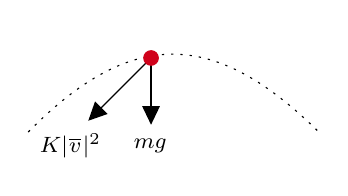
\begin{tikzpicture}[x=0.75pt,y=0.75pt,yscale=-1,xscale=1]
% Straight Lines [id:da989518658623866] 
\draw    (319.17,13.5) -- (319.17,42.67) ;
\draw [shift={(319.17,45.67)}, rotate = 270] [fill={rgb, 255:red, 0; green, 0; blue, 0 }  ][line width=0.08]  [draw opacity=0] (8.93,-4.29) -- (0,0) -- (8.93,4.29) -- cycle    ;
% Curve Lines [id:da2812861011221357] 
\draw  [dash pattern={on 0.84pt off 2.51pt}]  (260,49.17) .. controls (309.33,-0.83) and (349.33,-0.83) .. (400,49.17) ;
% Straight Lines [id:da6415802370859534] 
\draw    (291.04,41.63) -- (319.17,13.5) ;
\draw [shift={(288.92,43.75)}, rotate = 315] [fill={rgb, 255:red, 0; green, 0; blue, 0 }  ][line width=0.08]  [draw opacity=0] (8.93,-4.29) -- (0,0) -- (8.93,4.29) -- cycle    ;
% Shape: Circle [id:dp42638058294185255] 
\draw  [color={rgb, 255:red, 208; green, 2; blue, 27 }  ,draw opacity=1 ][fill={rgb, 255:red, 208; green, 2; blue, 27 }  ,fill opacity=1 ] (315.67,13.5) .. controls (315.67,11.57) and (317.23,10) .. (319.17,10) .. controls (321.1,10) and (322.67,11.57) .. (322.67,13.5) .. controls (322.67,15.43) and (321.1,17) .. (319.17,17) .. controls (317.23,17) and (315.67,15.43) .. (315.67,13.5) -- cycle ;

\draw (318.83,56) node [font=\footnotesize] {$mg$};
\draw (280.33,56) node [font=\footnotesize] {$K\vert \:\! \overline{v} \:\! \vert^{2}$};

\end{tikzpicture}
\end{center}


\noindent
Newton's Second Law of Motion states that the sum of forces $\vec{F}$ acting on an object is equal to the mass of the object, $m$, multiplied by the acceleration of the object, $\vec{a}$.
$$m\vec{a} = m\vec{g} - K\abs{\vec{v}}\vec{v}$$

\noindent
Let $\vec{s}(t) = [s_x(t), s_y(t)]^\top$ be the displacement vector of the cannonball from the origin at a given time $t$. By writing $\vec{a} = \vec{s}\;''$ and rearranging, we get the following system of second order ODEs.

$$
\begin{bmatrix}
	\matrixspacinghack s''_x(t) \\
	\matrixspacinghack s''_y(t) 	
\end{bmatrix}
=
\begin{bmatrix}
	\matrixspacinghack 0 \\
	\matrixspacinghack -9.8	
\end{bmatrix}
-
\frac{K}{m}\sqrt{s'_x(t)^2 + s'_y(t)^2}
\begin{bmatrix}
	\matrixspacinghack s'_x(t) \\
	\matrixspacinghack s'_y(t)	
\end{bmatrix} \\
$$


\noindent
The initial conditions for our system of ODEs is given by
$$s(0) = \begin{bmatrix} 0 \\ 0 \end{bmatrix} \quad \text{and} \quad s'(0) = \begin{bmatrix} v_0 \cos \theta \\ v_0 \sin \theta \end{bmatrix}$$

\noindent
As MATLAB's ODE solver, \lstinline|ode45|, only solves first order ODEs of the form $z' = f(t, z)$, we must reduce our second order system to a first order system. In order to do this, we define $z = [s_x(t), s_y(t), v_x(t), v_y(t)]^\top$ where $s_x, s_y$ are the component-wise displacement functions and $v_x, v_y$ are the component-wise velocity functions, and rewrite the system of equations as follows.

$$
z' = 
\begin{bmatrix}
	\matrixspacinghack s_x \\
	\matrixspacinghack s_y \\
	\matrixspacinghack v_x \\
	\matrixspacinghack v_y
\end{bmatrix}'
=
\begin{bmatrix}
	\matrixspacinghack v_x \\
	\matrixspacinghack v_y \\
	\matrixspacinghack -\frac{K}{m} v_x \sqrt{v_x^2 + v_y^2} \\
	\matrixspacinghack - g -\frac{K}{m} v_y \sqrt{v_x^2 + v_y^2}
\end{bmatrix}
$$

\noindent
The initial conditions for our first order system is given by
$$z(0) = \begin{bmatrix} s_x(0) \\ s_y(0) \\ v_x(0) \\ v_y(0) \end{bmatrix} = \begin{bmatrix} 0 \\ 0 \\ 450 \cos \theta \\ 450 \sin \theta \end{bmatrix}$$

\noindent
Finally, the implementation of the first order system in MATLAB is as follows.

\begin{lstlisting}
function s = projection_ode(t, z, g, m, K)
  s = zeros(4, 1);
  s(1) = z(3);
  s(2) = z(4);
  s(3) = -K * sqrt(z(3)^2 + z(4)^2) * z(3) / m;
  s(4) = -g - K * sqrt(z(3)^2 + z(4)^2) * z(4) / m;
end
\end{lstlisting}

%%%%%%%%%%%%%%%%%%%%%%%%%%%%%%%%%%%%%%%%%%%%%%%%%%%%%%%%%%%%
% Determining the point of impact with the ground
%%%%%%%%%%%%%%%%%%%%%%%%%%%%%%%%%%%%%%%%%%%%%%%%%%%%%%%%%%%%
\newpage
\subsection{Determining the point of impact with the ground}
First, we observe that the method signature of \lstinline|ode45| is
\begin{lstlisting}
[TOUT, YOUT, TE, YE, IE] = ode45(ODEFUN, TSPAN, Y0, OPTIONS)
\end{lstlisting}

\noindent
where \lstinline|TSPAN = [T0 FINAL]| is the interval of integration for our system of ODEs. However, the difficulty is that we wish to terminate the integration once the projectile touches the ground, but we do not know the time such event would occur beforehand. Instead, we can use an event function which will terminate the integration once the projectile touches the ground, which is exactly when $s_y = 0$. We can write the events function as follows.

\begin{lstlisting}
function [value, isTerminal, direction] = events_function(t, z)
  value = z(2);             % When the height is 0,
  isTerminal = 1;           % terminate integration,
  direction = -1;           % but only if the ball is falling
end
\end{lstlisting}

\noindent
However, \lstinline|TSPAN = [T0 FINAL]| is a required parameter of \lstinline|ode45|, regardless of whether we provide an event function. We can derive an upper bound on the duration of flight by calculating the flight time for the model with no air resistance, which is given by
$$\frac{2v_0 \sin\theta}{g}$$
where $v_0$ is the initial velocity and $\theta$ is the firing angle. As $2v_0 \sin\theta / g$ is bounded from above by $2v_0 / g$, we will use \lstinline|TSPAN = [0, 2 * v / g]| for the interval of integration.


%%%%%%%%%%%%%%%%%%%%%%%%%%%%%%%%%%%%%%%%%%%%%%%%%%%%%%%%%%%%
% Solving the system of equations
%%%%%%%%%%%%%%%%%%%%%%%%%%%%%%%%%%%%%%%%%%%%%%%%%%%%%%%%%%%%

\subsection{Solving the system of equations}
\noindent
We will create a function \lstinline|projection_solution(g, v, m, K, theta)| which returns the solution to our initial value problem, as follows.

\begin{lstlisting}
function [t, z, te, ze] = projection_solution(g, v, m, K, theta)
  ode = @(t, z) projection_ode(t, z, g, m, K);
  tspan = [0, 2 * v / g];
  ic = [0, 0, v * cos(theta), v * sin(theta)];
  options = odeset('events', events_function, 'reltol', 1e-8);
  [t, z, te, ze] = ode45(ode, tspan, ic, options);
end
\end{lstlisting}

$ $\\
\noindent
\textbf{Question:} In the absence of friction force, the maximum horizontal displacement can be calculated explicitly, given by the launch angle $\theta = \pi / 4$. What is the maximum horizontal distance and the associated angle, if we consider the above friction force?
